%----------------------------------------------------------------------------------------
%	PACKAGES AND OTHER DOCUMENT CONFIGURATIONS
%----------------------------------------------------------------------------------------

\documentclass[paper=a4, fontsize=11pt]{article} % A4 paper and 11pt font size

\usepackage[utf8x]{inputenc} % Use 8-bit encoding that has 256 glyphs
\usepackage[francais]{babel} % English language/hyphenation
\usepackage{amsmath,amsfonts,amsthm} % Math packages
\usepackage[margin=1in]{geometry}
\usepackage{sectsty} % Allows customizing section commands
\allsectionsfont{ \normalfont\scshape} % Make all sections centered, the default font and small caps
\subsectionfont{ \normalfont \underline} % Make all sections centered, the default font and small caps

\usepackage{fancyhdr} % Custom headers and footers
\pagestyle{fancyplain} % Makes all pages in the document conform to the custom headers and footers
\fancyhead{} % No page header - if you want one, create it in the same way as the footers below
\fancyfoot[L]{} % Empty left footer
\fancyfoot[C]{} % Empty center footer
\fancyfoot[R]{\thepage} % Page numbering for right footer
\renewcommand{\headrulewidth}{0pt} % Remove header underlines
\renewcommand{\footrulewidth}{0pt} % Remove footer underlines
\setlength{\headheight}{13.6pt} % Customize the height of the header

\numberwithin{equation}{section} % Number equations within sections (i.e. 1.1, 1.2, 2.1, 2.2 instead of 1, 2, 3, 4)
\numberwithin{figure}{section} % Number figures within sections (i.e. 1.1, 1.2, 2.1, 2.2 instead of 1, 2, 3, 4)
\numberwithin{table}{section} % Number tables within sections (i.e. 1.1, 1.2, 2.1, 2.2 instead of 1, 2, 3, 4)

\setlength\parindent{0pt} % Removes all indentation from paragraphs - comment this line for an assignment with lots of text

\usepackage[siunitx]{circuitikz}




%----------------------------------------------------------------------------------------
%	TITLE SECTION
%----------------------------------------------------------------------------------------

\newcommand{\horrule}[1]{\rule{\linewidth}{#1}} % Create horizontal rule command with 1 argument of height

\title{	
	\vspace{5cm}
	\normalfont \normalsize 
	\textsc{Universit\'e catholique de Louvain} \\ [25pt] % Your university, school and/or department name(s)
	\horrule{2pt} \\[0.4cm] % Thin top horizontal rule
	\huge LELEC 1530  \\ Syllabus d'exercice \\% The assignment title
	\horrule{2pt} \\[0.5cm] % Thick bottom horizontal rule
	\vspace{2cm}
	\centering
	
\includegraphics[width=4cm]{figure/Logo_UCL_DEF_cadre_EPL_RVB.jpg}
}

\author{} % Your name
\date{} % Today's date or a custom date

\setcounter{secnumdepth}{0} % sections are level 1

\begin{document}


\newcommand{\vtn}{$V_{T0,n}$ }
\newcommand{\vtp}{$V_{T0,p}$ }
\newcommand{\vin}{$V_{IN}$ }
\newcommand{\vout}{$V_{OUT}$ }
\newcommand{\vov}{$V_{OV}$ }
\newcommand{\ids}{$I_{DS}$ }
\newcommand{\vdd}{$V_{DD}$ }
\newcommand{\vgs}{$V_{GS}$ }
\newcommand{\cgs}{$C_{GS}$ }
\newcommand{\cgd}{$C_{GD}$ }
\newcommand{\vbe}{$V_{BE}$ }
\newcommand{\veb}{$V_{EB}$ }
\newcommand{\vge}{$V_{GE}$ }
\newcommand{\vcc}{$V_{CC}$ }
\newcommand{\voutun}{$V_{OUT,1}$ }
\newcommand{\voutdeux}{$V_{OUT,2}$ }
\newcommand{\vea}{$V_{EA}$ }
\newcommand{\cox}{$C_{ox}$ }

\pagenumbering{gobble}
\maketitle
\newpage
\null\newpage
\pagenumbering{roman}
\tableofcontents
\newpage
\pagenumbering{arabic}

\part{}
\setcounter{section}{1}
\section{Séance 1\\ MOSFET : polarisation}
\subsection*{Exercice 1}
Indiquez la caractéristique de sortie de l'amplificateur à la figure \ref{fig1-1}. Plus précisément on vous demande de tracer les courbe $V_{out}=f(V_{IN})$ ainsi que la droite de charge sur la courbe $i_{SD}/v_{SD}$ et d'indiquer les régimes de fonctionnement du transistor Q1 sur ces courbes. \\$V_{DD}$=5 V et R=5 k$\Omega$. Pour le transistor, $V_{T0,p}$=-0.8 V.

\begin{figure}[!htbp]
   \centering
   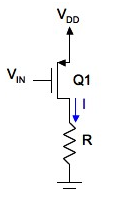
\includegraphics[]{figure/fig1-1.png}
   \caption{Exercice 1}
   \label{fig1-1}
\end{figure}

\subsection*{Exercice 2}
Soit le circuit suivant de la figure \ref{fig1-3}. Les paramètres technologiques sont : $k_{n}=1.2\times10^{-5}$ $A/V^2$, $V_{T0,n}$ =1 V, $V_{T0,p}$=-1 V et $k_{p}=0.4\times 10^{-5}$ $A/V^2$. On suppose , $\lambda$=0 et n=1.

\begin{figure}[!htbp]
   \centering
   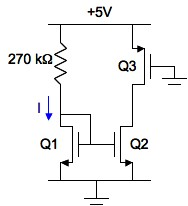
\includegraphics[]{figure/fig1-3.png}
   \caption{Exercice 3}
   \label{fig1-3}
\end{figure}

\begin{enumerate}
\item Calculez le courant I.
\item Calculez le courant dans branche de droite.
\item Calculez la tension $V_{D2}$.
\item Donnez le régime de fonctionnement des transistors. Qu'observez vous pour le transistor Q1?
\end{enumerate}

\subsection*{Exercice 3}
La figure \ref{fig1-2} représente un convertisseur courant - tension. Le courant d'entrée $I_{in}$ est transformé en une tension de sortie $V_{OUT}$. $V_{BIAS}$ est une tension constante. Les valeurs
des paramètres à utiliser sont les suivantes : $V_{DD}$=5 V, k1=k2=$3.9\times 10^5$ $A/V^2$, $V_{T0,n}$=1 V, $\lambda$=0 et n=1.

\begin{figure}[!htbp]
   \centering
   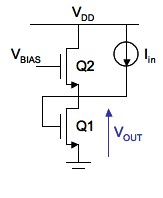
\includegraphics[]{figure/fig1-2.png}
   \caption{Exercice 2}
   \label{fig1-2}
\end{figure}

\begin{enumerate}
\item Expliquez le principe de fonctionnement de ce circuit.
\item Donnez le régime de fonctionnement des transistors en fonction de la valeur de $I_{in}$.
\item Quelles sont les valeurs minimales et maximales de $I_{in}$ ($I_{in}$ $<$ 0) pour lesquelles la caractéristique courant - tension est linéaire ? Utilisez la valeur $V_{BIAS}$ = 4 V.
\item Représentez la caractéristique $V_{OUT}$ = f($I_{in}$). Donnez l'équation de cette caractéristique en dehors de la plage de fonctionnement linéaire. Utilisez la valeur $V_{BIAS}$ = 4 V.
\item  Pour quelle valeur de $V_{BIAS}$ la plage de fonctionnement linéaire est-elle la plus large ?
\item  Que se passe-t-il si k1 est différent de k2 (i.e. la taille des transistors est différente) ? Justifiez.
\end{enumerate}















\newpage
\setcounter{section}{2}
\setcounter{figure}{0}
\section{Séance 2\\ MOSFET : petit signal}
\subsection*{Exercice 1}
Calculez le point de fonctionnement du circuit de la figure \ref{fig2-1}. Dimensionnez $V_{IN}$ et $(W/L)_n$ pour avoir une dynamique de sortie de 2V (c-à-d un $\Delta$\vout max de 2V ). Déterminez le gain du circuit pour cette valeur et les impédances d'entrées et de sortie du montage. Utilisez les paramètres technologiques suivants : $\mu_P$=0.04 m/V.s, $\mu_N$=0.1 m/V.s, $C_{OX}$=$10^-3$ F/m, $(W/L)_P$=1, n=1, $\lambda$ =0.02 $V^-1$, $V_{T0,n}$=1 V, $V_{T0,p}$=-1 V.
\begin{figure}[!htbp]
   \centering
   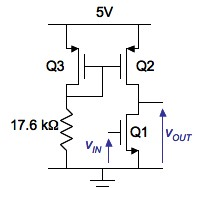
\includegraphics[]{figure/fig2-1.png}
   \caption{Exercice 1}
   \label{fig2-1}
\end{figure}



\subsection*{Exercice 2}
La figure 2 représente un amplificateur dont on étudie le comportement si $V_{IN}$ est augmenté. On considère que $V_{T0,n}$=1 V et que $k_n$=2 $mA/V^2$. On néglige l'effet Early dans un premier temps.
\begin{figure}[!htbp]
   \centering
   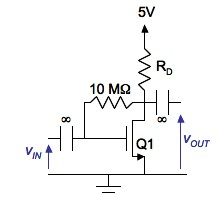
\includegraphics[]{figure/fig2-2.png}
   \caption{Exercice 2}
   \label{fig2-2}
\end{figure}
\begin{enumerate}
\item Montrez que le gain vaut : $\frac{V_{OUT}}{V_{IN}} = -\left(\frac{8}{V_{OV}}-2\right)$
où $V_{OV}=V_{GS}-V_{T0,n}$. Calculez $V_{GS}$, $I_{DS}$, gm, RD, et le gain si $V_{OV}$ est
compris entre 0.1 et 1 V ainsi que les impédances d'entrées et de sortie du montage.
\item Si $\lambda$ =0.02 $V{^-1}$, donnez une approximation de RD pour obtenir un gain de -10.
\end{enumerate}
\subsection*{Exercice 3}
Sur le circuit de la figure \ref{fig2-3}, le transistor NMOS possède un \vtn=0.9 V et $\lambda$ =0.02 $V^-1$ pour une tension VD=2 V. Que vaut le gain en tension \vout/\vin et les impédances d'entrées et de sortie du montage? Que deviennent VD et le gain si I est monté à 1 mA ?
\begin{figure}[!htbp]
   \centering
   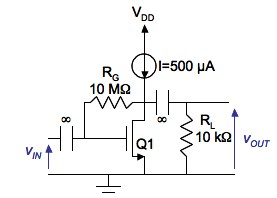
\includegraphics[]{figure/fig2-3.png}
   \caption{Exercice 3}
   \label{fig2-3}
\end{figure}



















\newpage
\setcounter{figure}{0}
\setcounter{section}{3}
\section{Séance 3\\ MOSFET : analyse fréquentielle}
\subsection*{Exercice 1}
L'amplificateur de la figure \ref{fig3-1} est polarisé pour fonctionner à \ids=1 mA pour un gm=1 mA/V.
\begin{figure}[!htbp]
   \centering
   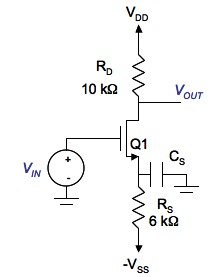
\includegraphics[]{figure/fig3-1.png}
   \caption{Exercice 1}
   \label{fig3-1}
\end{figure}
\begin{enumerate}
	\item En négligeant $r_0$, calculez le gain dans la bande passante.
	\item Donnez l'expression de la fonction de transfert H(s)=\vout(s)/\vin(s).
	\item Dessinez le diagramme de Bode
	\item Quel est le gain de l'amplificateur en DC.
	
\end{enumerate}


\subsection*{Exercice 2}
Le circuit de la figure \ref{fig3-2} est un amplificateur CMOS qui comporte les spécifications suivantes : \vdd=5 V, $R_1$ = $R_2$ = 500 k$\Omega$, $R_4$=1 k$\Omega$, $k_n=4\times 10^-3$ A/$V^2$ et \vtn=1 V. La source \vin  est uniquement petit signal. On néglige dans un premier temps l'effet Early et on considère que n=1.

\begin{figure}[!htbp]
   \centering
   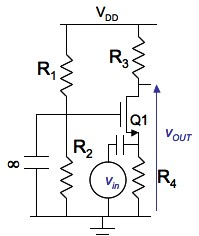
\includegraphics[]{figure/fig3-2.png}
   \caption{Exercice 2}
   \label{fig3-2}
\end{figure}

\begin{enumerate}
	\item Dimensionnez le $R_3$ et le transistor pour obtenir une dynamique maximale en sortie (c-a-d \vout = $\frac{V_{DD}}{2}$) et un courant \ids=1 mA.
	\item Pour $\lambda$=0,02 $V^-1$, donnez les expressions du gain dans la bande passante et des impédances d'entrée et de sortie.
	\item En tenant compte des capacités parasites \cgs=10 pF et \cgd=1 pF du transistor, évaluez sa bande passante.
\end{enumerate}
\newpage

\subsection*{Exercice 3}
La figure \ref{fig3-3} représente un amplificateur dit cascode replié.
\begin{figure}[!htbp]
   \centering
   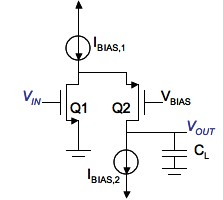
\includegraphics[]{figure/fig3-3.png}
   \caption{Exercice 3}
   \label{fig3-3}
\end{figure}

\begin{enumerate}
	\item Si les courants de polarisation sont tels que Q1 et Q2 ont des valeurs de gm et $r_0$ égales, et en supposant que la source $I_{BIAS,2}$ est implémentée de telle sorte qu'elle présente une impédance de sortie égale à l'impédance que cette source voit en regardant le drain de Q2, montrez que le gain vaut 0.5(gm$\times r_0$).
	\item Sachant que le pôle haute fréquence est habituellement formé au noeud de sortie, montrez que ce pôle vaut $\omega_H$=2/($C_L\times r_0$).
	\item Évaluez le gain et la fréquence de coupure du montage pour des valeurs de gm=0.5 mA/V, $r_0$=100 k$\Omega$ et $C_L$=1 pF.
\end{enumerate}















\newpage
\setcounter{figure}{0}
\setcounter{section}{4}
\section{Séance 4\\ BJT : polarisation et amplificateur}
\subsection*{Exercice 1}
Trois circuits à un transistor vous sont proposés à la figure \ref{fig4-1}.

\begin{figure}[!htbp]
   \centering
   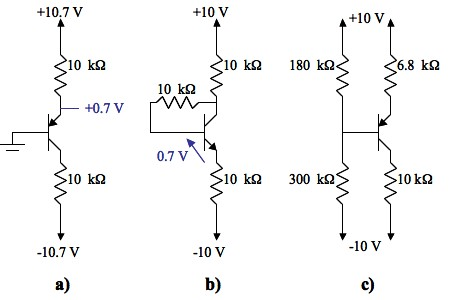
\includegraphics[]{figure/fig4-1.png}
   \caption{Exercice 1}
   \label{fig4-1}
\end{figure}

Pour ces circuits, donnez les valeurs des courants dans chaque branche ainsi que les tensions à chaque noeud. Considérez un gain $\beta$ très grand et que $|$\vbe$|$=0.7 V.

\subsection*{Exercice 2}
Le circuit de la figure \ref{fig4-2} est un amplificateur à deux transistors bipolaires. On vous demande de calculer le point de polarisation du circuit pour des valeurs de gain en courant valant respectivement :
\begin{enumerate}
\item $\beta$=$\infty$
\item $\beta$=100
\item $\beta$=10
\end{enumerate}
\begin{figure}[!htbp]
   \centering
   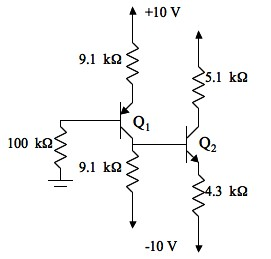
\includegraphics[]{figure/fig4-2.png}
   \caption{Exercice 2}
   \label{fig4-2}
\end{figure}

\newpage
\subsection*{Exercice 3}
La figure \ref{fig4-3} représente un amplificateur BJT utilisant un transistor PNP. On considère que \veb  est ajusté tel que $V_C$=8 V alors que \vcc=10 V, $R_C$=2 k$\Omega$ et qu'on applique un signal \veb=$0.004 sin(\omega t)$.

\begin{figure}[!htbp]
   \centering
   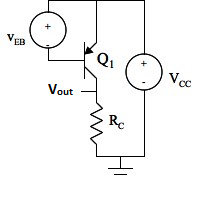
\includegraphics[]{figure/fig4-3.png}
   \caption{Exercice 3}
   \label{fig4-3}
\end{figure}

\begin{enumerate}
	 \item  Trouvez les quantités instantanées $i_B$(t), $i_C$(t) et $v_C$(t).
	 \item En considérant un gain de $\beta$=100 pour le transistor, que vaut le gain en tension ?
\end{enumerate}











\newpage
\setcounter{figure}{0}
\setcounter{section}{5}
\section{Séance 5\\ BJT : petit signal et analyse fréquentielle}

\subsection*{Exercice 1}
L'amplificateur de la figure \ref{fig5-1} est polarisé par une source de courant $I_E$ et possède un gain en courant $\beta$ très élevé.

\begin{figure}[!htbp]
   \centering
   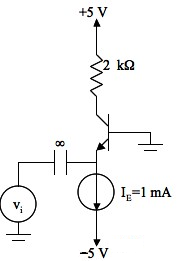
\includegraphics[]{figure/fig5-1.png}
   \caption{Exercice 1}
   \label{fig5-1}
\end{figure}

On vous demande de déterminer la tension $V_E$, $V_B$, $V_C$, gm et de remplacer le transistor par son modèle $\pi$-hybride. Calculez ensuite le gain en tension $V_c/V_i$.

\subsection*{Exercice 2}
Dans le circuit de la figure \ref{fig5-2}, on suppose que le transistor fonctionne en régime actif.
\begin{enumerate}
\item En supposant également que $\beta$ est grand, calculez le courant de collecteur du transistor.
\item Remplacez le transistor par son modèle équivalent petit signal en T, calculez les gains en tensions $V_{OUT,1}$/\vin et $V_{OUT,2}$/\vin.
\end{enumerate}

\begin{figure}[!htbp]
   \centering
   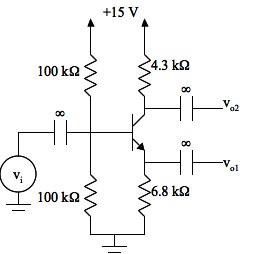
\includegraphics[]{figure/fig5-2.png}
   \caption{Exercice 2}
   \label{fig5-2}
\end{figure}

\newpage
\subsection*{Exercice 3}
Pour le transistor de la figure \ref{fig5-3}, on vous donne : $R_S$=$R_L$=1 k$\Omega$, $\beta$=100, $f_T$=400 MHz et $C_\mu$=2 pF. Pour rappel, $f_T=\frac{gm}{2\pi(C_\pi+C_\mu)}$

\begin{figure}[!htbp]
   \centering
   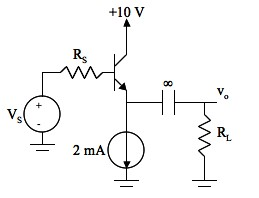
\includegraphics[]{figure/fig5-3.png}
   \caption{Exercice 3}
   \label{fig5-3}
\end{figure}

\begin{enumerate}
\item Déterminez le gain en bande passante.
\item Expliquez par rapport au modèle complet $\pi$-hybride, quels termes on peut négliger dans le calcul du pôle dû à la capacité $C_\mu$ et donnez-en l'expression simplifiée ainsi que sa valeur ?
\end{enumerate}













\newpage
\setcounter{figure}{0}
\setcounter{section}{6}
\section{Séance 6\\ MOSFET and BJT : petit signal et analyse fréquentielle}
\subsection*{Exercice 1}
L'amplificateur ci-dessous possède un gain en courant $\beta$=200 et une tension d'Early \vea infinie. $C_\pi$=2 pF et $C_\mu$=0.5 pF.

\begin{figure}[!htbp]
   \centering
   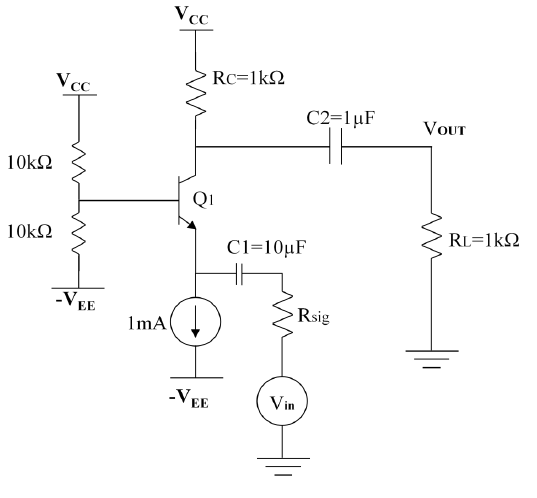
\includegraphics[]{figure/fig6-1.png}
   \caption{Exercice 1}
   \label{fig6-1}
\end{figure}

Pour les trois première questions, considérez que $C_1$ et $C_2$ sont des capacités de découplage et négligez $R_sig$.
\begin{enumerate}
\item De quelle structure d'ampli s'agit 'il ?
\item Quel est le gain en tension \vout/\vin du circuit ?
\item Déterminez le pôle haute fréquence
	\item Calculez les pôles basse fréquences si $R_{sig}$ = 10 $\Omega$
 \item Tracez le diagramme de Bode
\end{enumerate}

\newpage
\subsection*{Exercice 2}
Le circuit de la figure 2 est un amplificateur CMOS qui comporte les spécifications suivantes : $C_1$=10nF, $C_2$=1$\mu$F considérées comme des capacités de découplage, $R_L$=1k$\Omega$, $R_{inv}$=50$\Omega$ et $R_G$=10M$\Omega$ et gm =0.1.
La source \vin est uniquement petit signal et la tension d'Early \vea est très grande.

\begin{figure}[!htbp]
   \centering
   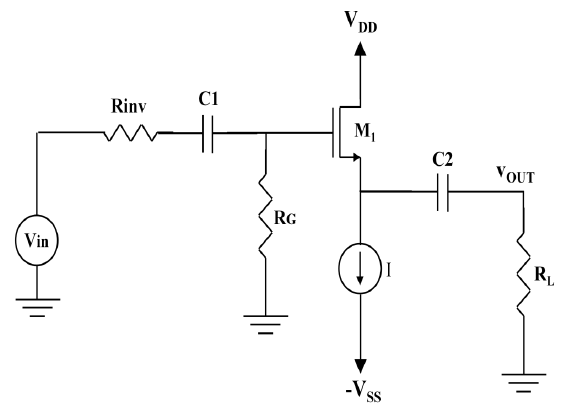
\includegraphics[]{figure/fig6-2.png}
   \caption{Exercice 2}
   \label{fig6-2}
\end{figure}

\begin{enumerate}
\item De quel type d'ampli est composée la figure \ref{fig6-2}? quel est son gain approximatif sans calcul ?
\item Donnez les expressions du gain dans la bande passante et des impédances d'entrée et de sortie.
\item En tenant compte des capacités internes \cgs=101 pF et \cgd=9 pF du transistor, évaluez le pôle haute fréquence
\item Calculez les pôles basse fréquence
\item Tracez le diagramme de Bode du circuit
\end{enumerate}



































\newpage
\part{}
\setcounter{figure}{0}
\setcounter{section}{7}

\section{Séance 7\\ Logique digitale de base}
\subsection*{Exercice 1 : modèles digitaux}

\begin{figure}[!htbp]
   \centering
   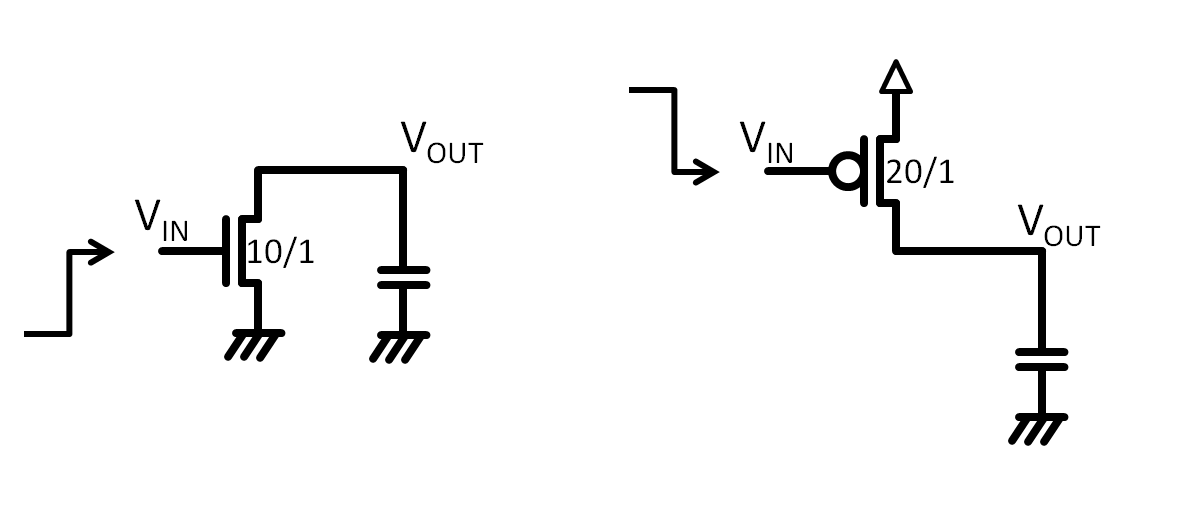
\includegraphics[width=10cm]{figure/fig7-1.png}
   \caption{Exercice 1}
   \label{fig7-1}
\end{figure}

Calculez les délais à 50\% des transitions symbolisées sur la figure~\ref{fig7-1}
pour des transistors à canaux court en technologie 50nm avec \cox=62.5aF/$\mu m^2$,
$R_n$=34k$\Omega\mu$m et $R_p$=68k$\Omega\mu$m.
Les tailles des NMOS valent $W=10\mu$m et $L=1\mu$m tandis que celles des PMOS valent
$W=20\mu$m et $L=1\mu$m.

\subsection*{Exercice 2 : inverseur CMOS}

On considère une chaîne d'inverseurs CMOS identiques avec ses pistes d'interconnexion
en technologie 0.18$\mu$m, comme représenté à la figure~\ref{fig7-2}. Voici les paramètres
technologiques :

\begin{center}
$
	\begin{array}{l l l}
		L_{min} = 0.18 \mu m 	& V_{DD} = 1.8 V 		& V_{t0,n} = |V_{t0,p} | = 0.5 V \\
		\mu_n = 0.04 m^2/Vs 	& \mu_p = 0.02 m^2/Vs	& C_{ox} = 5 fF/\mu m^2 \\
		C_{rout} = 10fF			&						& \\
	\end{array}
$
\end{center}

\begin{figure}[!htbp]
   \centering
   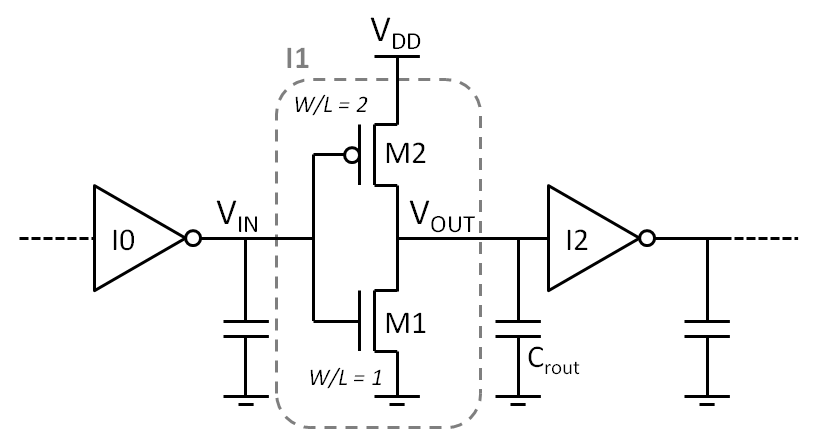
\includegraphics[width=10cm]{figure/fig7-2.png}
   \caption{Exercice 1}
   \label{fig7-2}
\end{figure}

\emph{Analyse DC}
\begin{enumerate}
	\item Pour une transition infiniment lente à l'entrée de I1, déterminez le régime de
	fonctionnement de M1 et M2 ainsi que la tension \vout en fonction de \vin.
\end{enumerate}

\emph{Délai de propagation}
\begin{enumerate}
	\setcounter{enumi}{1}
	\item Comme estimation du délai de propagation ($t_p$) de I1, on vous demande de
	calculer le temps de descente de \vout à 50\% lors d'un flanc montant sur \vin
	($t_{PHL}$). Pour ce faire, remplacer M1 et M2 par des éléments plus simples
	(résistance, sources) en fonction du régime de fonctionnement. On suppose que
	le flanc sur \vin est idéal et on néglige les capacités parasites.
	\item On souhaite simplifier le calcul du délai de propagation en remplaçant M1
	par une résistance équivalente $R_{eq}$ qui donne la même valeur de délai que
	celle trouvée précédemment. Pour ce faire, on vous demande de trouver un facteur
	de fitting k pour exprimer $R_{eq}$ en fonction de la résistance en mode linéaire
	:\\ $R_{eq}$ = k $R_{lin}$ .
\end{enumerate}

\emph{Scaling de la technologie CMOS}
\begin{enumerate}
	\setcounter{enumi}{3}
	\item On considère cette fois une technologie 65nm avec les paramètres ci-dessous.
	Calculer le délai sur base de la formule obtenue au point c). Négliger les capacités parasites.

	\begin{center}
	$
		\begin{array}{l l l}
			L_{min} = 65 nm 		& V_{DD} = 1.2V 		&V_{t0,n} = |V_{t0,p}| = 0.4V \\
			\mu_n = 0.05 m^2/Vs 	& \mu_p= 0.025 m^2/Vs	& C_{ox} = 7 fF/\mu m^2 \\
			C_{rout} = 2fF			&						& \\
		\end{array}
	$
	\end{center}
\end{enumerate}

\subsection*{Exercice 3 : Logique de passage}
On considère les 3 implémentations d'un multiplexeur 2 vers 1 de la figure~\ref{fig7-3} :
transmission gate, pass gate et static CMOS gate. La fonction logique associée est :
Y = (Sel.A) + ($\overline{Sel}$.B) et la technologie considérée est une technologie
0.18 $\mu$m avec les paramètres suivants:

\begin{center}
$
	\begin{array}{l l l}
		L_{min} = 0.18 \mu m 	& V_{DD} = 1.8 V 		& V_{t0,n} = |V_{t0,p} | = 0.5 V \\
		\mu_n = 0.04 m^2/Vs 	& \mu_p = 0.02 m^2/Vs	& C_{ox} = 5 fF/\mu m^2 \\
		C_{rout} = 10fF			&						& \\
	\end{array}
$
\end{center}

\begin{figure}[!htbp]
   \centering
   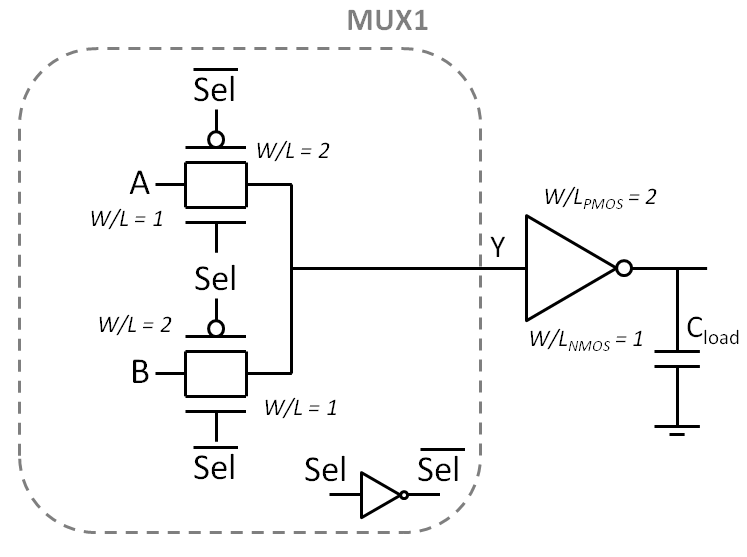
\includegraphics[width=9cm]{figure/fig7-3-1.png}
	 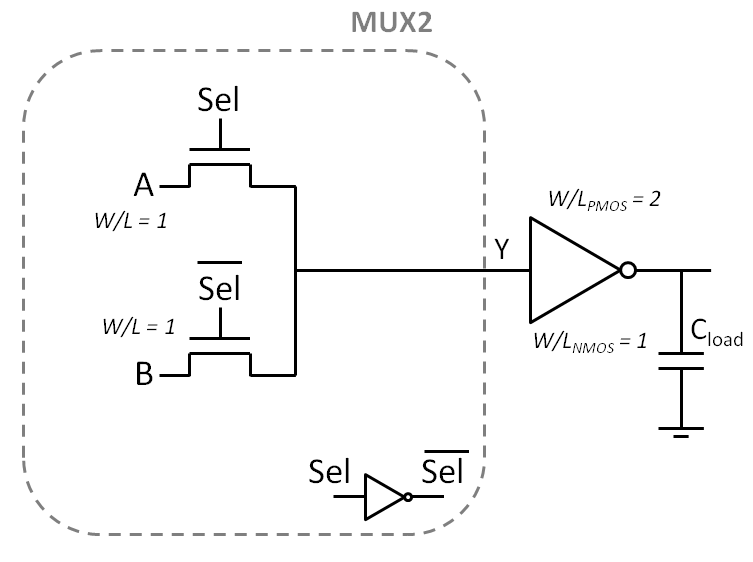
\includegraphics[width=9cm]{figure/fig7-3-2.png}
	 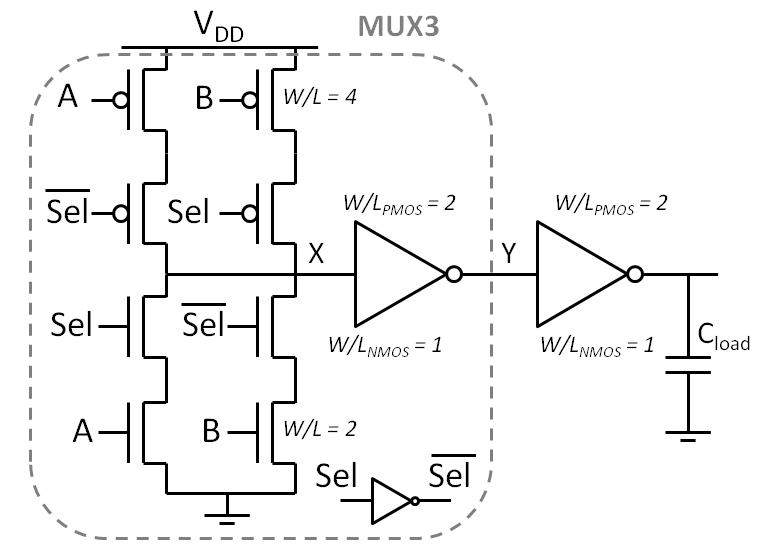
\includegraphics[width=9cm]{figure/fig7-3-3.png}
   \caption{Exercice 1}
   \label{fig7-3}
\end{figure}

\begin{enumerate}
	\item Déterminer les tensions des niveaux logiques haut ($V_{OH}$) et bas ($V_{OL}$) de
	la sortie Y pour chacun de ces multiplexeurs.
	\item Calculez le temps de décharge à 50\% ($t_{PHL}$) de la capacité $C_{load}$ par
	l'inverseur de l'étage suivant, suite à un flanc montant à la sortie Y. Considérez une
	résistance équivalente pour les transistors passant du régime saturé au linéaire de
	$R_{eq}$ = 2.5 $R_{lin}$ et négliger toutes les capacités parasites.
\end{enumerate}


\newpage
\setcounter{figure}{0}
\setcounter{section}{8}
\section{Séance 8\\ Portes logiques CMOS}
\subsection*{Exercice 1 : Circuit combinatoire}
Quelle est la fonction implémentée par le circuit représenté à la figure \ref{fig8-1} ?
\begin{figure}[!htbp]
   \centering
   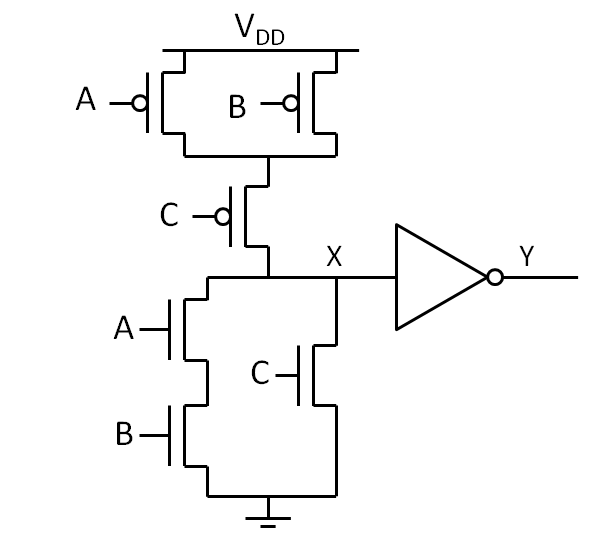
\includegraphics[width=7cm]{figure/fig8-1.png}
   \caption{Exercice 1}
   \label{fig8-1}
\end{figure}

\subsection*{Exercice 2 : Porte combinatoire}

On désire construire une porte logique qui implémente la fonction suivante Y = $\overline{A.(B+C)}$ dans une technologie 50nm.
\begin{enumerate}
	\item Proposez un schéma d'implémentation basé sur des transistors MOS.
	\item Proposez un dimensionnement des transistors qui donnera un courant de sortie similaire à celui de l'inverseur unitaire ($L_{min}$=50nm, $W_{n}$=500nm, $W_{p}$=1000nm).
\item Calculer le temps de montée de la sortie à 50\% ($t_{PLH}$) en considérant une résistance équivalente pour les transistors passant du mode saturé au mode linéaire de $R_N$=34/W k$\Omega$ et RP=68/W k$\Omega$ et en considérant \cox=$62.5\times W \times L$ aF. Une capacité de load $C_L$ = 50fF est ajoutée au noeud Y.
\end{enumerate}

\subsection*{Exercice 3: Logique dynamique}
On considère le circuit en logique dynamique de la Fig\ref{fig8-3} dans une technologie 50nm. Voici les paramètres technologiques :
\begin{center} $ \begin{array}{l l l l} L_{min} = 50nm & C_{ox} = 62.5\times W \times L aF & R_N=34/W k \Omega & R_P=68/W k\Omega\\ \end{array}$\end{center}

\begin{figure}[!htbp]
   \centering
   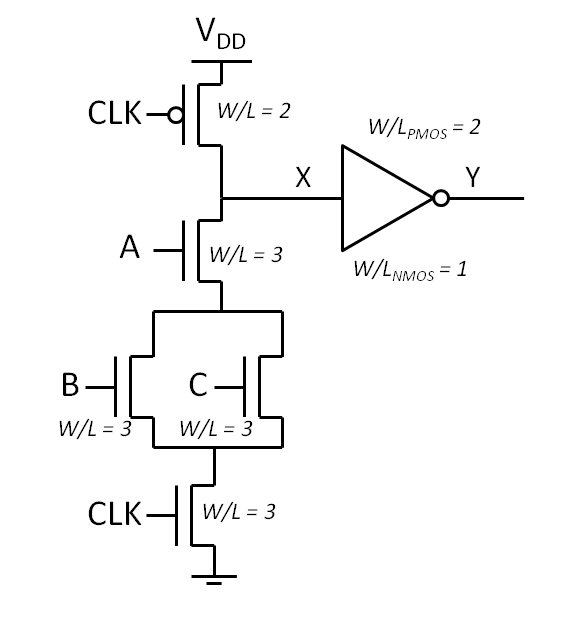
\includegraphics[width=8cm]{figure/fig8-3.png}
   \caption{Exercice 1}
   \label{fig8-3}
\end{figure}

\begin{enumerate}
\item Expliquer le principe de fonctionnement de ce circuit. Quelle est la fonction logique implémentée ?
\item Dans cette technologie les transistors NMOS ont un courant de fuite de 1nA/$\mu$m à \vgs=0V. Calculer pendant combien de temps la sortie Y restera valide suite à un flanc montant sur CLK quand B=C=1 et que A=0.
\item Comment conserver le niveau logique sur le noeud X à l'aide d'un transistor supplémentaire ?
\end{enumerate}

\newpage
\subsection*{Exercice 4 : DFF}
On considère le master d'un D-Flip Flop présenté à la Figure \ref{fig8-4} dans une technologie 50nm. Voici les paramètres technologiques :
\begin{center} $ \begin{array}{l l l l} L_{min} = 50nm & C_{ox} = 62.5\times W \times L\text{ aF} & R_N=34/W k \Omega& R_P=68/W k\Omega\\ \end{array}$\end{center}

\begin{figure}[!htbp]
   \centering
   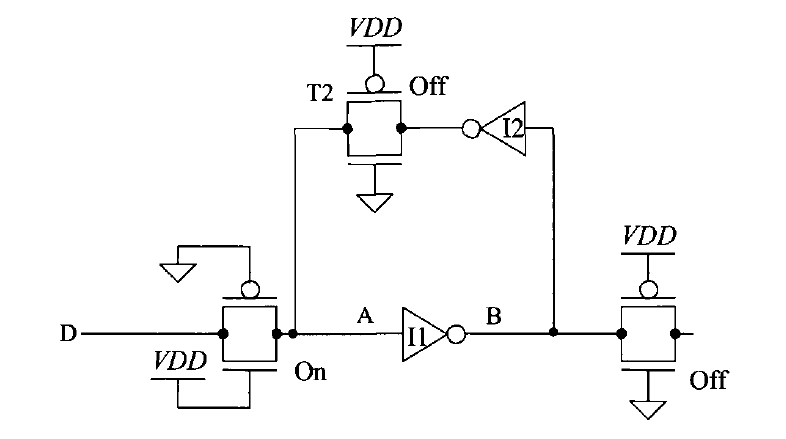
\includegraphics[width=10cm]{figure/fig8-4.png}
   \caption{Exercice 1}
   \label{fig8-4}
\end{figure}

\begin{enumerate}
\item Calculez les capacités aux noeuds A et B.
\item Calculez les délais entre les noeuds D et A et entre les noeuds A et B.
\end{enumerate}







\newpage
\setcounter{figure}{0}
\setcounter{section}{9}
\section{Séance 9\\Sources de courant}
\subsection*{Exercice 1 : Résistance de sortie cascode}
Calculez la résistance de sortie du montage ci-dessous. Le transistor est un transistor canal long de (W/L)=10/2. Utilisez les données de la table 9.1 du cours pour obtenir les valeurs numériques.

\begin{figure}[!htbp]
   \centering
   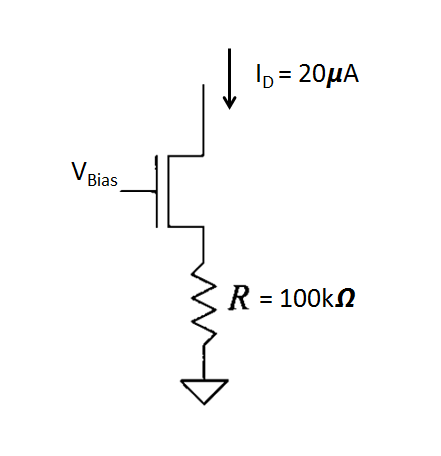
\includegraphics[width=5cm]{figure/fig10-1.png}
   \caption{Exercice 1}
   \label{fig10-1}
\end{figure}

\subsection*{Exercice 2 : Miroir de courant cascodé}
On considère le miroir de courant cascodé de la Figure \ref{fig10-2} dans une technologie canal long 1?$\mu$m. Les paramètres technologiques sont dans la table 9.1 du cours. NMOS : 50/2, PMOS : 100/2.
Déterminez la taille du transistor MWS pour que le transistor M3 soit saturé.

\begin{figure}[!htbp]
   \centering
   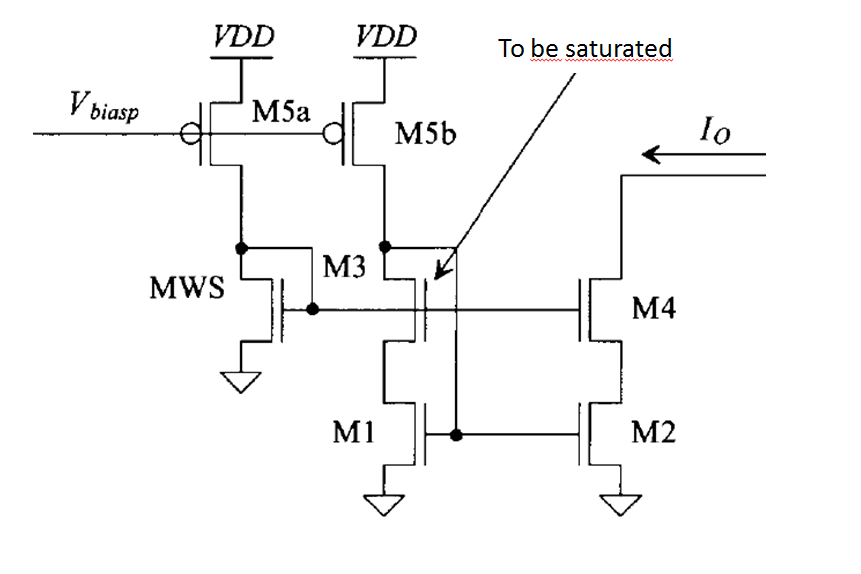
\includegraphics[width=10cm]{figure/fig10-2.png}
   \caption{Exercice 1}
   \label{fig10-2}
\end{figure}

\subsection*{Exercice 3 : source complexe}
On considère une source de courant complexe présenté à la Figure \ref{fig10-3} dans une technologie canal long (voir table 9.1 du cours). Calculez les courants et les tensions partout dans le circuit.

\begin{figure}[!htbp]
   \centering
   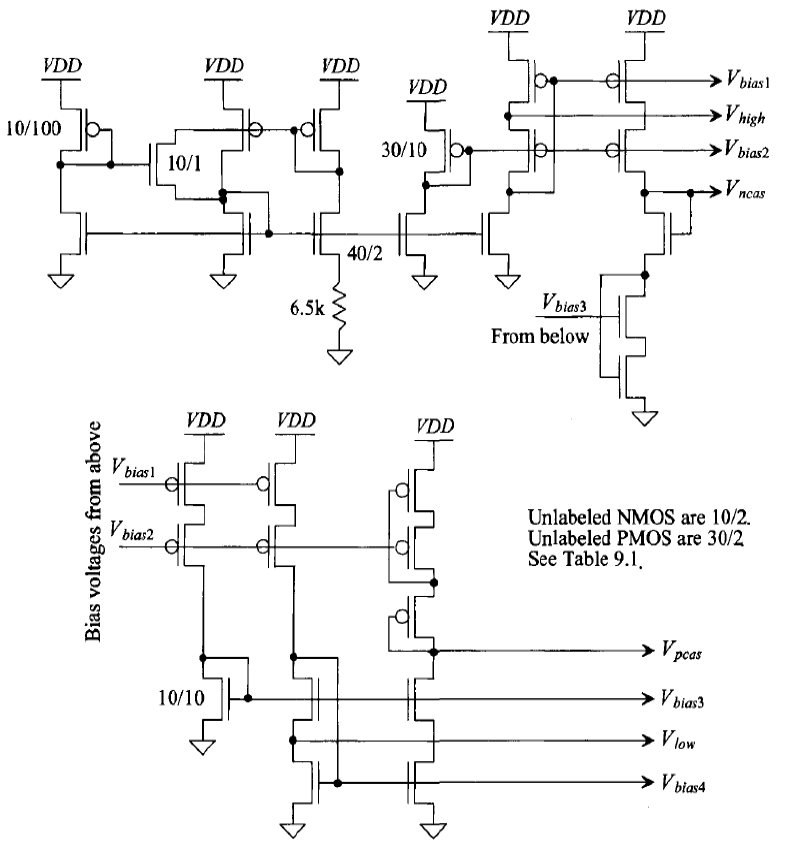
\includegraphics[width=18cm]{figure/fig10-3-bis.png}
   \caption{Exercice 1}
   \label{fig10-3}
\end{figure}
\newpage

\begin{figure}[!htbp]
   \centering
   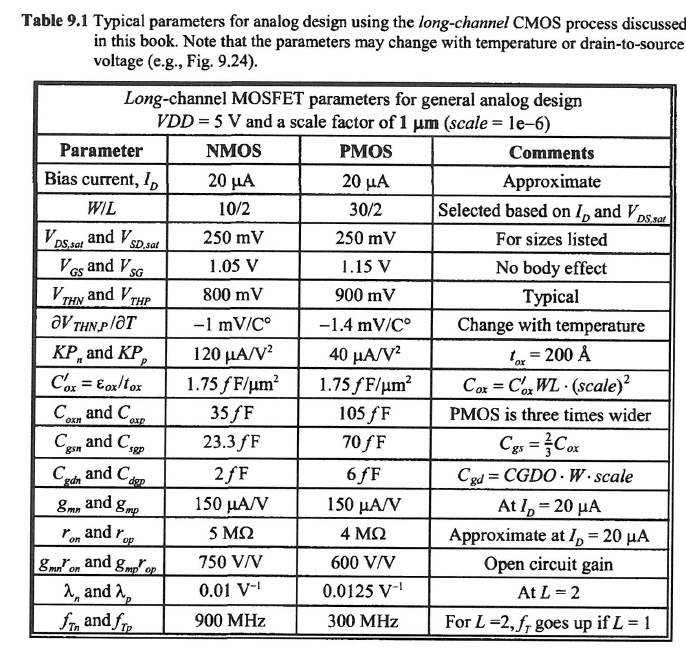
\includegraphics[width=18cm]{figure/table9-1.png}
   \caption{Table 9.1}
   \label{table9-1}
\end{figure}

















\newpage
\setcounter{figure}{0}
\setcounter{section}{10}
\section{Séance 10\\ Paire différentielle simple}
\subsection*{Exercice 1}
On considère la paire différentielle de la Figure \ref{fig11-1} avec :

$\begin{array}{l l l l l}KP_n = KP_p = 200?A/V^2&  V_A = 50V & V_T = 1V & V_{DD} = 5V & V_1 = V_2 = 0V\\ \end{array}$

\begin{figure}[!htbp]
   \centering
   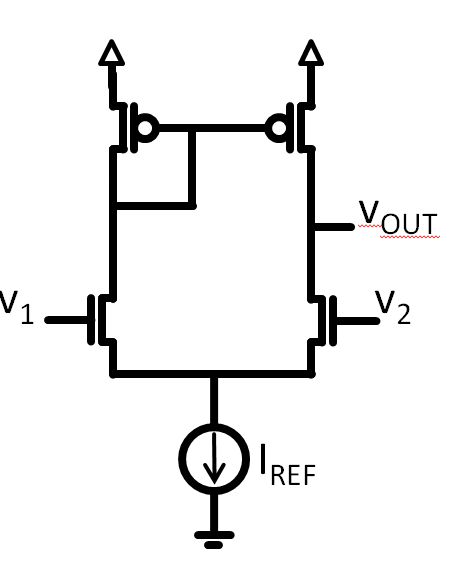
\includegraphics[width=5cm]{figure/fig11-1.png}
   \caption{Exercice 1}
   \label{fig11-1}
\end{figure}

\begin{enumerate}
\item  Pour $I_{ref}$ : 10 $\mu$A, calculez la dynamique de sortie de la paire, la transconductance des transistors d'entrée et la conductance d'Early des 4 transistors.
\item  Calculez la résistance de sortie de la paire différentielle
\item  Obtenez l'expression et la valeur du gain en tension de la paire par le principe de superposions.
\item  Reproduisez les résultats de a, b et c pour $I_{ref}$ : 100 $\mu$A.
\end{enumerate}

\subsection*{Exercice 2 : Paire différentielle complexe}

On considère la paire différentielle complexe de la Figure \ref{fig11-2} dans une technologie canal long 1?$\mu$m. Les paramètres technologiques sont dans la table 9.1 du cours. NMOS : 10/2, PMOS : 20/2. 
Obtenez l'expression analytique ainsi que la valeur du gain ($V_{out,+}-V_{out,-}$)/($V_{in,+}-V_{in,-}$).
\newpage
\begin{figure}[!htbp]
   \centering
   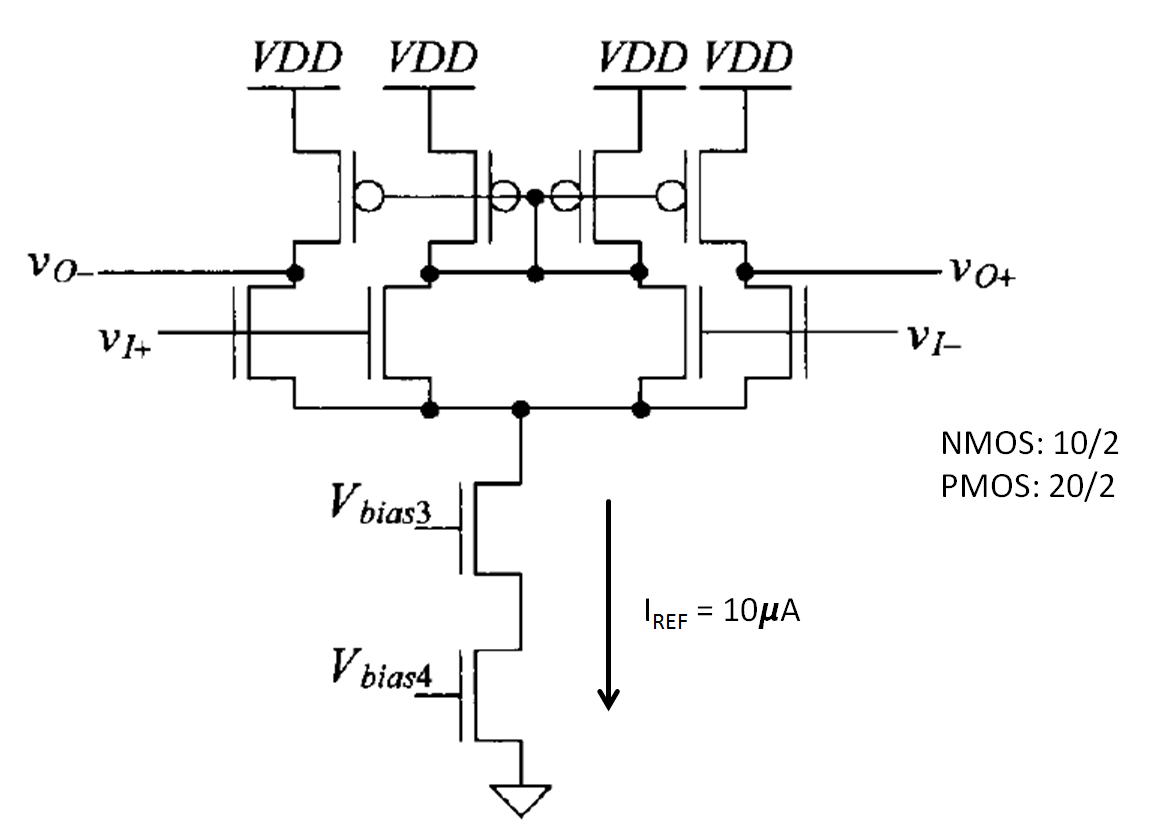
\includegraphics[width=10cm]{figure/fig11-2.png}
   \caption{Exercice 1}
   \label{fig11-2}
\end{figure}



















\newpage
\setcounter{figure}{0}
\setcounter{section}{11}
\section{Séance 11\\ Ampli Op}

\subsection*{Exercice 1 : paire différentielle}
\begin{figure}[!htbp]
   \centering
   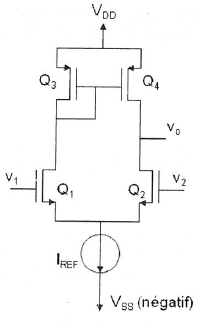
\includegraphics[]{figure/fig12-1-1.png}
   \caption{Exercice 1}
   \label{fig12-1-1}
\end{figure}

\begin{enumerate}
\item  Pour $I_{ref}$=10$\mu$A, calculez la plage linéaire de \vout, les valeurs de gm1 et gm2. 
\item que vaut l'impédance de sortie du montage et son  gain en tension?
\item Refaites les calculs pour $I_{ref}$=100$\mu$A et commentez.
\end{enumerate}

\subsection*{Exercice 2 : Amplificateur opérationnel}
On considère l'amplificateur de la Figure \ref{fig12-1} avec les paramètres technologiques de la table 9.1.
\begin{enumerate}
\item  Identifiez l'entrée négative.
\item  Identifiez les différents blocs qui constituent ce circuit, expliquez leur rôle.
\item  Donnez l'expression du gain différentiel dans la bande passante en fonction du rapport des tailles des transistors $Q_{5,6}$ par rapport aux transistors $Q_{3,4}$.
\item  Donnez les expressions des pôles et zéros dus aux capacités parasites ainsi qu'à $C_L$. Esquissez ensuite le diagramme de Bode.
\item  Soit $Q_{5,6}$ 4x plus grand que $Q_{3,4}$, $I_{REF}$=10$\mu$A, $(W/L)_{PMOS}$=50/4, $(W/L)_{NMOS}$=25/4 et $(W/L)_{PAIRE}$=100/2. calculez :
	\begin{itemize}
		\item La dynamique de sortie
		\item La valeur en mode commun maximale admissible aux entrées
		\item La résistance de sortie de l'amplificateur
		\item Le gain de l'amplificateur en bande passante
		\item La valeur des pôles et redessinez le diagramme de Bode
\end{itemize}

\end{enumerate}
\begin{figure}[!htbp]
   \centering
   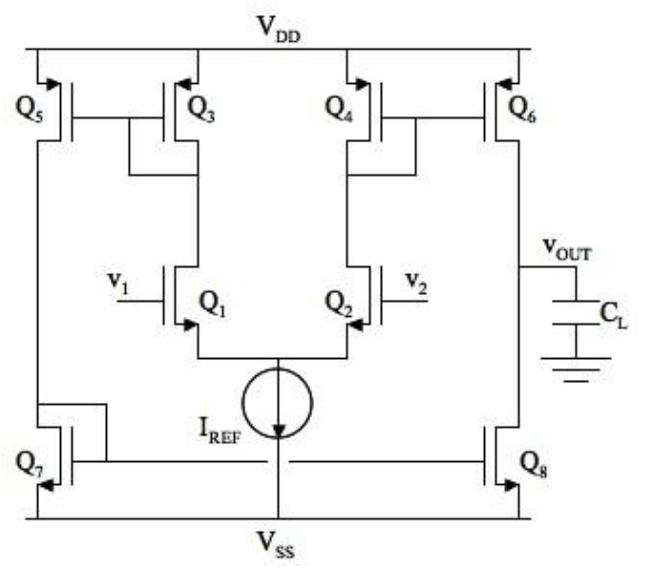
\includegraphics[width=10cm]{figure/fig12-1.png}
   \caption{Exercice 2}
   \label{fig12-1}
\end{figure}







\clearpage
\newpage
\setcounter{figure}{0}
\setcounter{section}{12}
\section{Exercices complémentaires}

\subsection*{Exercice 1}
On considère la source de courant de la Figure \ref{fig13-1} basée sur un miroir CMOS simple avec les paramètres suivants : \vdd=5V, k=200$\mu$A/$V^2$ et \vtn=1V.

\begin{figure}[!htbp]
   \centering
   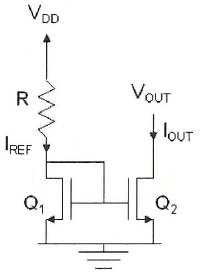
\includegraphics[]{figure/fig13-1.png}
   \caption{Exercice 1}
   \label{fig13-1}
\end{figure}

\begin{enumerate}
\item en considérant une largeur de canal W de 1$\mu$m et une longueur de canal L de 1$\mu$m pour $Q_1$, calculez la valeur de R pour obtenir un $I_{ref}$ de $100\mu$A.
\item Quelle est la tension \vout minimale pour que le montage fonctionne correctement?
\item Pour obtenir un $I_{out}$ de 1mA, on considère un (W/L) pour $Q_2$ de 10/1 en $\mu$m. Pour une tension d'Early \vea=20V/$\mu$m, calculez la résistance de sortie du montage ainsi que la variation de courant due à une augmentation de \vout de 1V.
\item Que deviennent ces valeurs pour une taille de $Q_2$ de 100/10 en $\mu$m (même courant $I_{out}$)?
\end{enumerate}


\subsection*{Exercice 2}
Le miroir de courant de la figure 1 est constitué de trois BJTs de type NPN dont le gain en courant $\beta$ est supposé infini.

\begin{figure}[!htbp]
   \centering
   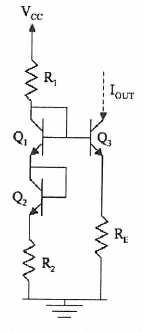
\includegraphics[]{figure/fig13-2.png}
   \caption{Exercice 2}
   \label{fig13-2}
\end{figure}

\begin{enumerate}
\item si $R_1$=$R_2$, démontrez que $I_{out}$ vaut: $I_{out} = \frac{V_{cc}}{2R_E}$
\item Si \vcc = 15V et que $I_{out}$=1mA, dimensionnez $R_E$
\item Quelle est la plus faible tension acceptable au collecteur de $Q_3$ pour que le circuit fonctionne correctement?
\end{enumerate}

\newpage
\subsection*{Exercice 3}
La figure \ref{fig13-3} représente une source en courant de Widlar. On suppose que $I_{ref}$ =100$\mu$A.

\begin{figure}[!htbp]
   \centering
   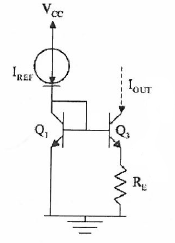
\includegraphics[]{figure/fig13-3.png}
   \caption{Exercice 3}
   \label{fig13-3}
\end{figure}

\begin{enumerate}
\item Si on désire fournir un courant de sortie de 10 $\mu$A avec un $\beta$ très grand, que doit valoir $R_E$?
\item A présent, considérons que $\beta$=200 et que la tension d'Early vaut \vea=100V. Que vaut l'impédance de sortie du montage ?
\end{enumerate}


\subsection*{Exercice 4 : Circuit combinatoire}
Implémentez et dimensionnez la fonction X = $\overline{ABCD}$ + E en logique domino et en CMOS sur base de l'inverseur unitaire ($L_{min}$=50nm, $W_n$=500nm, $W_p$=1000nm). Comparez la surface de silicium nécessaire à l'implémentation en ne comptant que la surface occupée par les transistors.

\subsection*{Exercice 5: Logique dynamique}
On considère le circuit en logique dynamique de la Figure \ref{fig9-2} dans une technologie 50nm. Voici les paramètres technologiques :
\begin{center} $ \begin{array}{l l l l} L_{min} = 50nm & C_{ox} = 62.5\times W \times L\text{ aF} & R_N=34/W k \Omega& R_P=68/W k\Omega\\ \end{array}$\end{center}

\begin{figure}[!htbp]
   \centering
   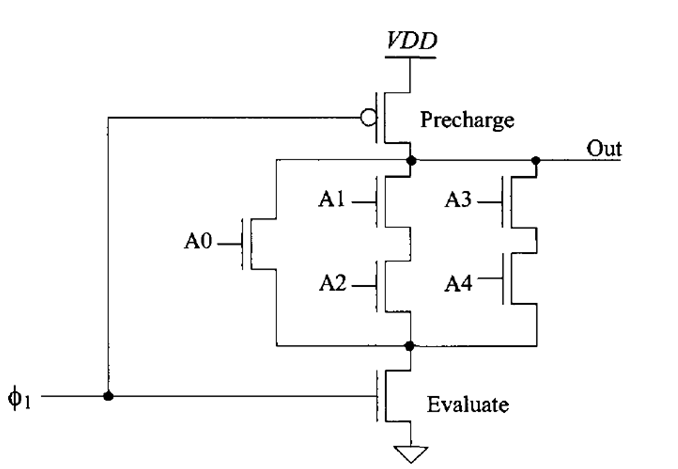
\includegraphics[width=14cm]{figure/fig9-2.png}
   \caption{Exercice 1}
   \label{fig9-2}
\end{figure}

\begin{enumerate}
\item Quelle est la fonction logique implémentée ?
\item Dimensionnez la porte par rapport à l'inverseur unitaire (Lmin=50nm, Wn=500nm Wp=1000nm).
\item Calculez le délai $t_{PHL}$ à 50\% lorsque $A_0$=1 et $A_{1->4}$=0.
\end{enumerate}

\subsection*{Exercice 6 : full adder}

On considère un additionneur sur 1bit présenté à la Figure \ref{fig9-3} dans une technologie 50nm. Voici les paramètres technologiques :
\begin{center} $ \begin{array}{l l l l} L_{min} = 50nm & C_{ox} = 62.5\times W \times L\text{ aF} & R_N=34/W k \Omega& R_P=68/W k\Omega\\ \end{array}$\end{center}

\begin{figure}[!htbp]
   \centering
   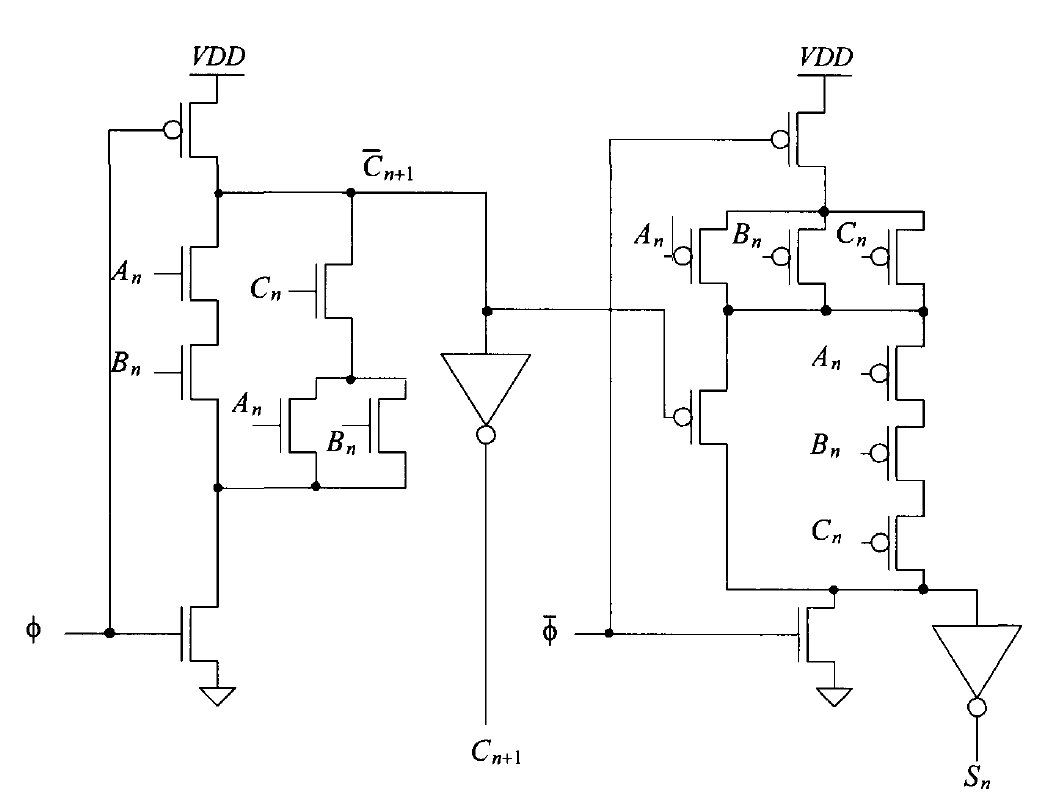
\includegraphics[width=13cm]{figure/fig9-3.png}
   \caption{Exercice 1}
   \label{fig9-3}
\end{figure}

\begin{enumerate}
\item  Décrivez le type de logique utilisé dans la Figure \ref{fig9-3}. Donnez la fonctionnalité logique de chacune des deux portes sous forme d'une table de vérité ainsi que la fonctionnalité logique globale.
\item  Dimensionnez les deux portes logique sur base de l'inverseur unitaire ($L_{min}$=50nm, $W_{n}$=500nm, $W_{p}$=1000nm).
\item  Implémentez un additionneur prenant en entrée des mots de 2 bits sur base de l'additionneur sur 1 bit de la Figure \ref{fig9-3}.
\item  Pour une fréquence de clock de 200MHz, combien de temps faut-il pour additionner 2 mots de 2bits ? Combien de temps faudrait-il si l'architecture implémente une addition sur 2 mots de 32bits ?
\end{enumerate}










\end{document}




